% !TEX root = ../Thesis.tex

\chapter{Theory}

\section{Electron Spin Resonance}
\subsection{Basic Theory}

Electron spin resonance (EPR) functions by detecting the energy difference between the spin states of an electron.
Normally degenerate, the presence of a magnetic field separates the two spin states parallel to it in energy.
The spin state parallel to the magnetic field has a lower energy whilst the anti-parallel state has a higher energy.
These are described as the up, $\ket{\uparrow}$, and down, $\ket{\downarrow}$, spin states.
For an electron in free space the energy difference is given by:

\begin{equation}
\Delta E = g_e\mu_bB,
\label{eq:enSplit}
\end{equation}

where $g_e$ is the free electron g-factor, $\mu_b$ is the Bohr magneton and $B$ is the magnetic field strength. 
This results in an energy splitting as seen in figure \ref{fig:elecSplit}. 

\begin{figure}
\centering
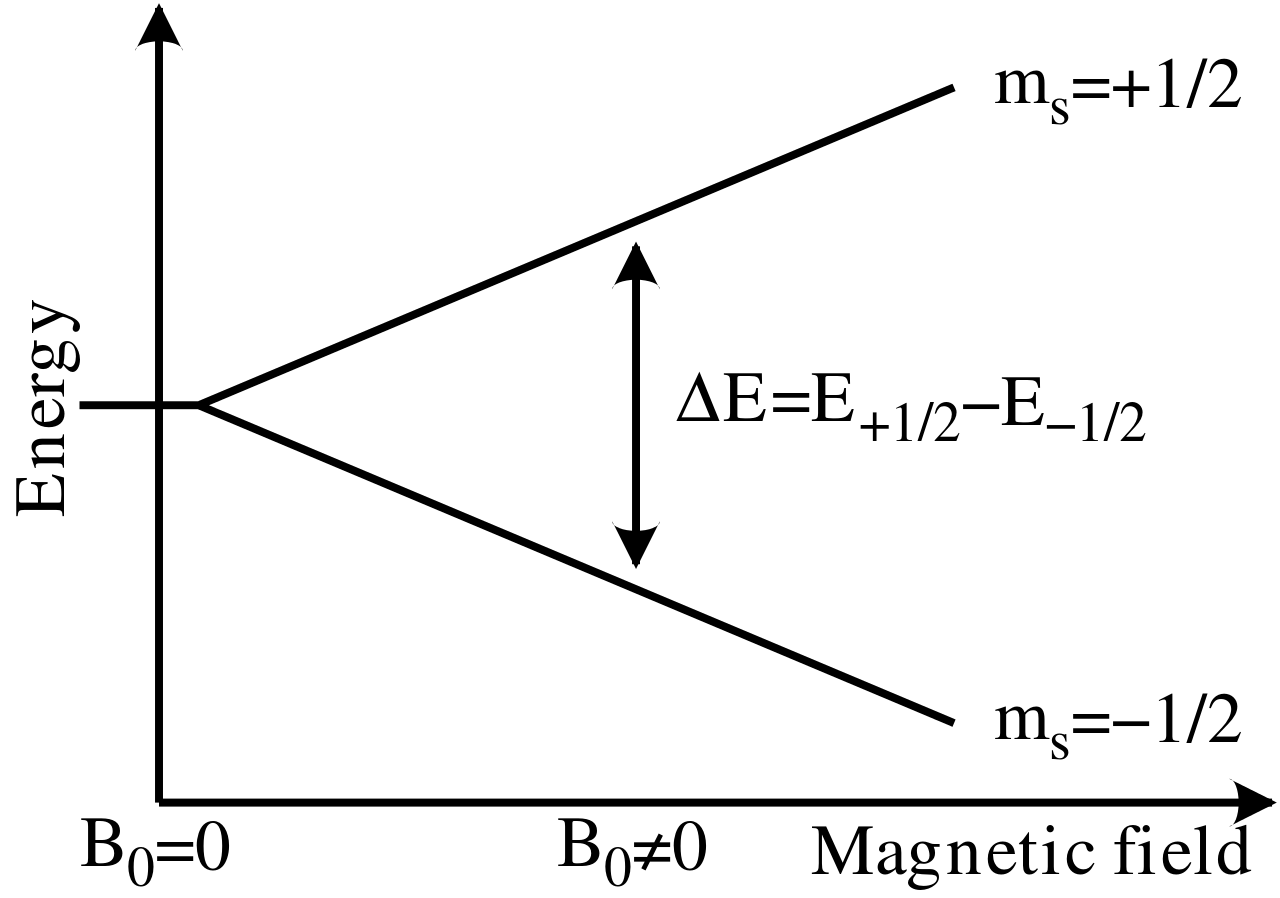
\includegraphics[width = 0.5\columnwidth]{Figures/EPR_splitting.png}
\caption[Free electron level splitting]{Spin state energy splitting for a free electron in a magnetic field.}
\label{fig:elecSplit}
\end{figure}

In practice this energy splitting can be detected using continuous wave EPR. Transitions between the spin states will be driven by incident electromagnetic radiation of photon energy equal to the energy gap (i.e $h\nu = g_e\mu_bB$). 
The presence of an EPR transition in a sample can be detected either by applying a constant magnetic field and sweeping EM frequency incident on that sample or vice versa.
In practice, it is the latter that is used for experimental simplicity.
Measuring reflection of radiation from the sample whilst sweeping magnetic field will reveal a drop in reflection at the transition field - when photons are absorbed by spins moving from the lower to higher energy state.

\subsection{Pulsed Electron Spin Resonance and Qubits}
The description above details continuous wave (CW) ESR, a technique that has proven invaluable for studying the electronic structure of materials.
Another ESR has proven more popular for the manipulation of spins for use of qubits: pulsed ESR.
This uses short bursts of microwave radiation, on resonance with the spin transition, to control spin states and allows the spin to function as a qubit.
Pulses are described in terms of a rotation angle, with a $\pi$ pulse taking  the ensemble of spins from the down to up state or vice versa. 
A $\pi/2$ pulse takes the spins into the plane normal to the magnetic field, termed the $x-y$ plane. 
This causes the spins to precess in the magnetic field at the Lamor frequency given by:
\begin{equation}
\label{eq:larmor}
\omega = \frac{eg}{2m}B_0
\end{equation}

\subsubsection{Hahn Echo and Detection}

In pulsed ESR the spins are detected via the electromagnetic radiation they emit when precessing in a magnetic field. 
This radiation is of the same frequency as the resonant control radiation (easily shown using equations \ref{eq:enSplit} and \ref{eq:larmor}).
This emitted radiation can be demodulated with the control radiation giving a DC signal.
In a perfectly homogeneous magnetic field all spins would precess at the same rate giving a constant DC signal but in reality all spins will precess at slightly different rates due to small, static differences in the magnetic field each experiences.
So, following a $\pi/2$ pulse, the signal from the spins will rapidly decay as the ensemble of spins lose phase coherence. 
A technique, known as a spin or Hahn echo, to reverse this loss of phase was developed by Erwin Hahn in 1950 \cite{hahn1950}. 
This follows a $\pi/2$ pulse with a $\pi$ pulse after a set time interval, $T$. 
\textit{Static} magnetic field differences now act to reverse the loss of phase coherence. 
This results in a brief re-phasing of the spins following another interval $T$, detected as a rise and fall of a DC signal or and 'Echo'.
A cartoon of this sequence is shown in figure \ref{fig:HahnEcho}. 

\begin{figure}
\centering
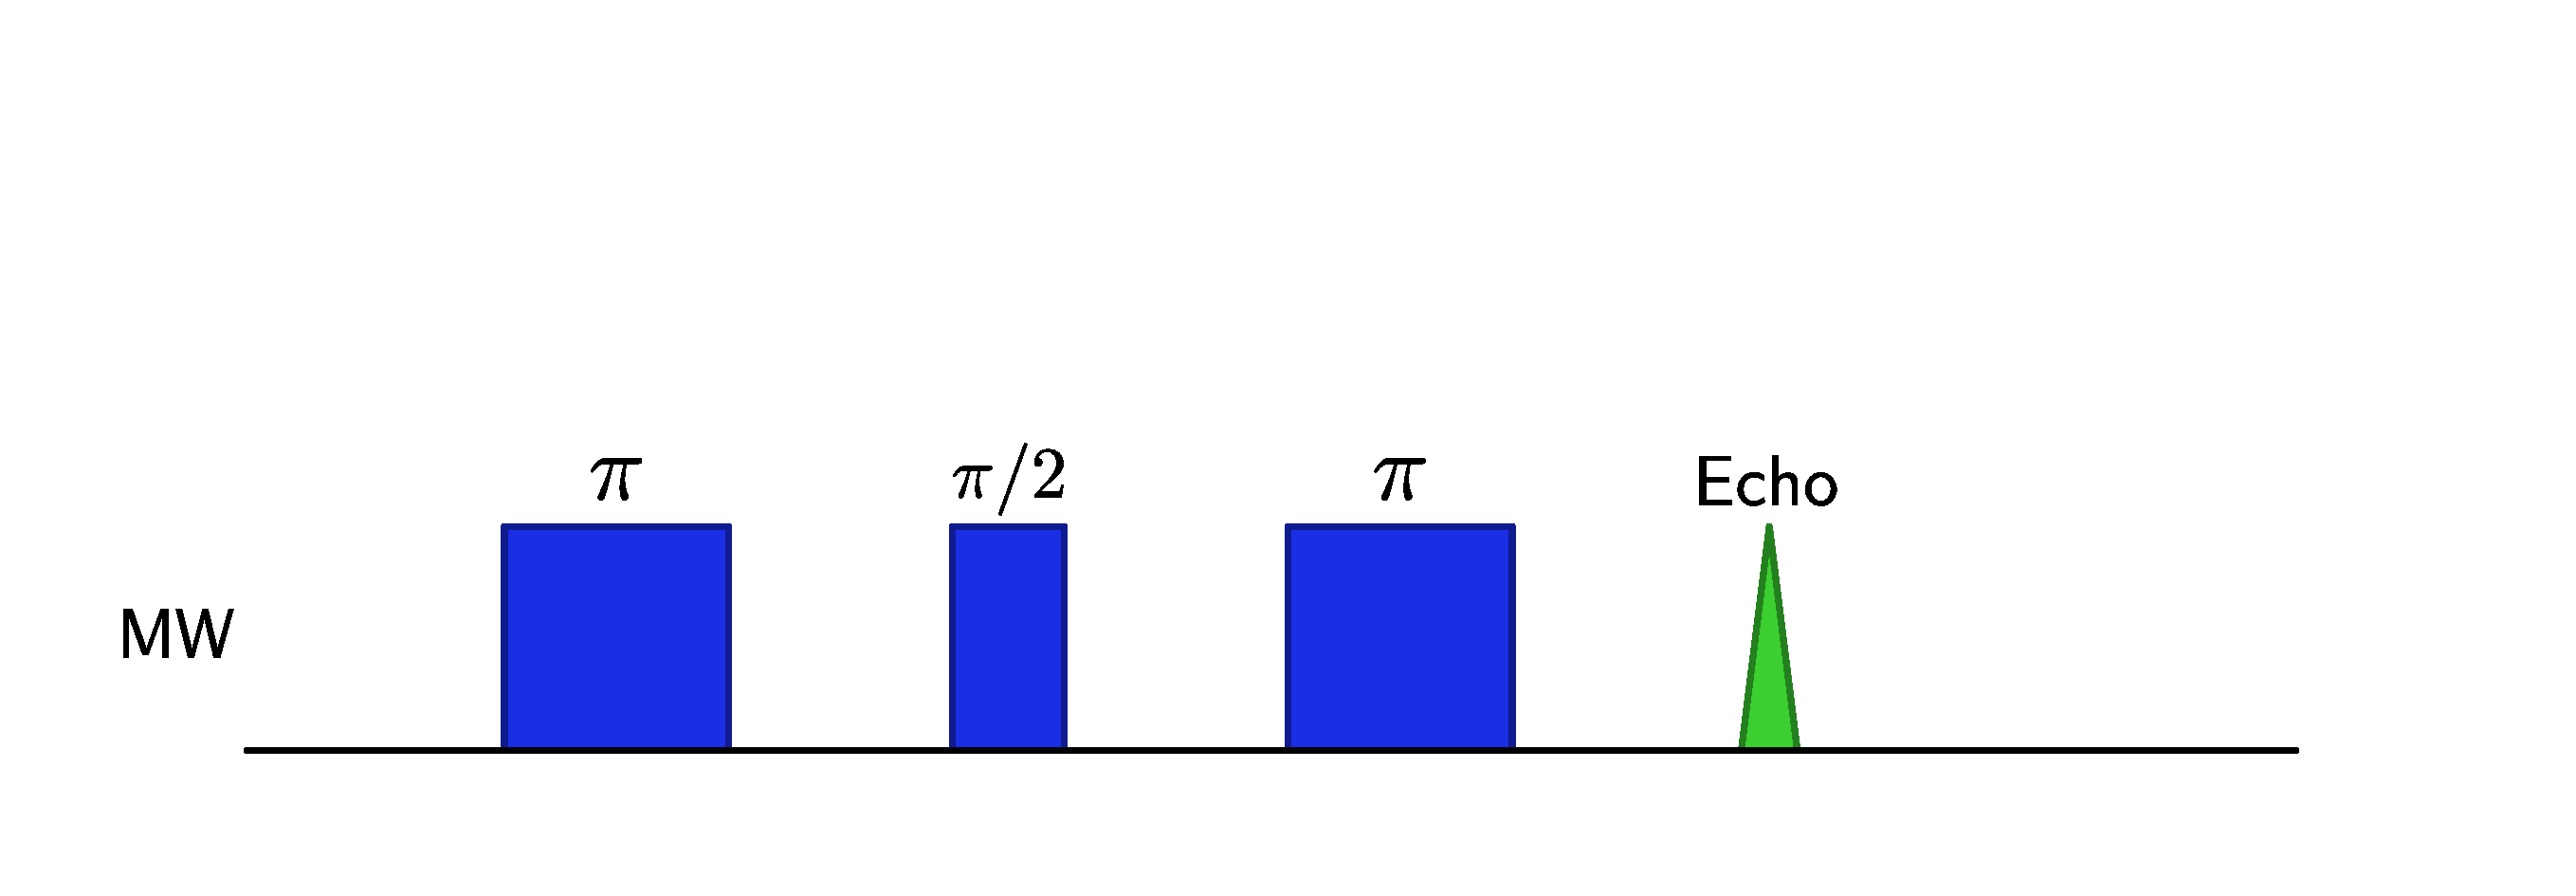
\includegraphics[width = \columnwidth]{Figures/hahnEcho.pdf}
\caption[Hahn echo sequence]{Cartoon showing a Hahn echo pulse sequence. A $\frac{\pi}{2}$ pulse causes the spins to precess in the $x-y$ plane. Loss of phase coherence is reversed via a $\pi$ pulse following time interval $T$ and a signal is detected following another interval of $T$.}
\label{fig:HahnEcho}
\end{figure}